\documentclass[12pt,twoside]{article}

\usepackage[backend=biber,style=alphabetic]{biblatex} 
\addbibresource{ref.bib}  


%%%%%%%%%%%%%%%%%%%%%%%%%%%%%%%%%%%%%%%%%%%%%%%%%%%%%%%%%%%%%%%%%%%%%%%%%%%%%

% Definitions for the title page
% Edit these to provide the correct information
% e.g. \newcommand{\reportauthor}{Timothy Kimber}

\newcommand{\reporttitle}{An idigital interface designed for sharing diagnostic medical imaging with patients}
\newcommand{\reportauthor}{Laura Hagege LH}
\newcommand{\supervisor}{Fernando Bello}
\newcommand{\degreetype}{Msc. Computing Science}

%%%%%%%%%%%%%%%%%%%%%%%%%%%%%%%%%%%%%%%%%%%%%%%%%%%%%%%%%%%%%%%%%%%%%%%%%%%%%

% load some definitions and default packages
%%%%%%%%%%%%%%%%%%%%%%%%%%%%%%%%%%%%%%%%%
% University Assignment Title Page 
% LaTeX Template
% Version 1.0 (27/12/12)
%
% This template has been downloaded from:
% http://www.LaTeXTemplates.com
%
% Original author:
% WikiBooks (http://en.wikibooks.org/wiki/LaTeX/Title_Creation)
%
% License:
% CC BY-NC-SA 3.0 (http://creativecommons.org/licenses/by-nc-sa/3.0/)
% 
%
%%%%%%%%%%%%%%%%%%%%%%%%%%%%%%%%%%%%%%%%%
%----------------------------------------------------------------------------------------
%	PACKAGES AND OTHER DOCUMENT CONFIGURATIONS
%----------------------------------------------------------------------------------------
\usepackage[a4paper,hmargin=2.8cm,vmargin=2.0cm,includeheadfoot]{geometry}
\usepackage{textpos}
\usepackage{natbib} % for bibliography
\usepackage{tabularx,longtable,multirow,subfigure,caption}%hangcaption
\usepackage{fncylab} %formatting of labels
\usepackage{fancyhdr} % page layout
\usepackage{url} % URLs
\usepackage[english]{babel}
\usepackage{amsmath}
\usepackage{graphicx}
\usepackage{dsfont}
\usepackage{epstopdf} % automatically replace .eps with .pdf in graphics
\usepackage{backref} % needed for citations
\usepackage{array}
\usepackage{latexsym}
\usepackage[pdftex,pagebackref,hypertexnames=false,colorlinks]{hyperref} % provide links in pdf

\hypersetup{pdftitle={},
  pdfsubject={}, 
  pdfauthor={},
  pdfkeywords={}, 
  pdfstartview=FitH,
  pdfpagemode={UseOutlines},% None, FullScreen, UseOutlines
  bookmarksnumbered=true, bookmarksopen=true, colorlinks,
    citecolor=black,%
    filecolor=black,%
    linkcolor=black,%
    urlcolor=black}

\usepackage[all]{hypcap}


%\usepackage{color}
%\usepackage[tight,ugly]{units}
%\usepackage{float}
%\usepackage{tcolorbox}
%\usepackage[colorinlistoftodos]{todonotes}
% \usepackage{ntheorem}
% \theoremstyle{break}
% \newtheorem{lemma}{Lemma}
% \newtheorem{theorem}{Theorem}
% \newtheorem{remark}{Remark}
% \newtheorem{definition}{Definition}
% \newtheorem{proof}{Proof}


%%% Default fonts
\renewcommand*{\rmdefault}{bch}
\renewcommand*{\ttdefault}{cmtt}



%%% Default settings (page layout)
\setlength{\parindent}{0em}  % indentation of paragraph

\setlength{\headheight}{14.5pt}
\pagestyle{fancy}
\renewcommand{\chaptermark}[1]{\markboth{\chaptername\ \thechapter.\ #1}{}} 

\fancyfoot[ER,OL]{\sffamily\textbf{\thepage}}%Page no. in the left on odd pages and on right on even pages
\fancyfoot[OC,EC]{\sffamily }
\renewcommand{\headrulewidth}{0.1pt}
\renewcommand{\footrulewidth}{0.1pt}
\captionsetup{margin=10pt,font=small,labelfont=bf}


%--- chapter heading

\def\@makechapterhead#1{%
  \vspace*{10\p@}%
  {\parindent \z@ \raggedright \sffamily
    \interlinepenalty\@M
    \Huge\bfseries \thechapter \space\space #1\par\nobreak
    \vskip 30\p@
  }}

%---chapter heading for \chapter*  
\def\@makeschapterhead#1{%
  \vspace*{10\p@}%
  {\parindent \z@ \raggedright
    \sffamily
    \interlinepenalty\@M
    \Huge \bfseries  #1\par\nobreak
    \vskip 30\p@
  }}

\allowdisplaybreaks

% load some macros
% Here, you can define your own macros. Some examples are given below.

\newcommand{\R}[0]{\mathds{R}} % real numbers
\newcommand{\Z}[0]{\mathds{Z}} % integers
\newcommand{\N}[0]{\mathds{N}} % natural numbers
\newcommand{\C}[0]{\mathds{C}} % complex numbers
\renewcommand{\vec}[1]{{\boldsymbol{{#1}}}} % vector
\newcommand{\mat}[1]{{\boldsymbol{{#1}}}} % matrix


\date{September 2018}

\begin{document}

% load title page
% Last modification: 2015-08-17 (Marc Deisenroth)
\begin{titlepage}

\newcommand{\HRule}{\rule{\linewidth}{0.5mm}} % Defines a new command for the horizontal lines, change thickness here


%----------------------------------------------------------------------------------------
%	LOGO SECTION
%----------------------------------------------------------------------------------------


\includegraphics[width = 4cm]{./figures/imperial}\\[0.5cm] 

\center % Center remainder of the page

%----------------------------------------------------------------------------------------
%	HEADING SECTIONS
%----------------------------------------------------------------------------------------

\textsc{\Large Imperial College London}\\[0.5cm] 
\textsc{\large Department of Computing}\\[0.5cm] 

%----------------------------------------------------------------------------------------
%	TITLE SECTION
%----------------------------------------------------------------------------------------

\HRule \\[0.4cm]
{ \huge \bfseries \reporttitle}\\ % Title of your document
\HRule \\[1.0cm]

%----------------------------------------------------------------------------------------
%	SUB TITLE SECTION
%----------------------------------------------------------------------------------------

\textsc{\large --- Background and Progress Report ---}\\[0.5cm] 
 
%----------------------------------------------------------------------------------------
%	AUTHOR SECTION
%----------------------------------------------------------------------------------------



\emph{by} \\
\reportauthor % Your name

~

\emph{Supervisor:} 
\supervisor % Supervisor's Name




%----------------------------------------------------------------------------------------
%	FOOTER & DATE SECTION
%----------------------------------------------------------------------------------------
\vfill % Fill the rest of the page with whitespace
Submitted in partial fulfillment of the requirements for the MSc degree in
\degreetype~of Imperial College London\\[0.5cm]

\makeatletter
\@date 
\makeatother


\end{titlepage}



% page numbering etc.
%\pagenumbering{roman}
%\clearpage{\pagestyle{empty}\cleardoublepage}
%\setcounter{page}{1}
%\pagestyle{fancy}

%%%%%%%%%%%%%%%%%%%%%%%%%%%%%%%%%%%%
%\begin{abstract}
%Your abstract.
%\end{abstract}

%\cleardoublepage
%%%%%%%%%%%%%%%%%%%%%%%%%%%%%%%%%%%%
%\section*{Acknowledgments}
%Comment this out if not needed.

\clearpage{\pagestyle{empty}\cleardoublepage}

%%%%%%%%%%%%%%%%%%%%%%%%%%%%%%%%%%%%
\begin{abstract}
\normalsize



"The abstract is a very brief summary of the report's contents. It should be about half page long. Somebody unfamiliar with your project should have a good idea of what it is about having read the abstract alone and will know whether it will be of interest to them."

\end{abstract}
\clearpage


%%%%%%%%%%%%%%%%%%%%%%%%%%%%%%%%%%%%
\renewcommand{\abstractname}{Acknowledgements}
\begin{abstract}

"It is usual to thank those individuals who have provided particularly useful assistance, technical or otherwise, during your project. Your supervisor will obviously be pleased to be acknowledged as they will have invested quite a lot of time overseeing your progress."

Person to thank:
\newline \vspace{5mm}
- I would like to express my deep gratitude to Professor Dr Fernando Bello
\newline \vspace{5mm}
- Will Cox
\newline \vspace{5mm}
- Co-workers at Chelsea and westminster hospital
\newline \vspace{5mm}
- Developper community over the internet and around me 
\newline \vspace{5mm}



\end{abstract}
\clearpage


%%%%%%%%%%%%%%%%%%%%%%%%%%%%%%%%%%%%
%--- table of contents
%\fancyhead[RE,LO]{\sffamily {Table of Contents}}
\tableofcontents 

\clearpage{\pagestyle{empty}\cleardoublepage}
\pagenumbering{arabic}
\setcounter{page}{1}
\fancyhead[LE,RO]{\slshape \rightmark}
\fancyhead[LO,RE]{\slshape \leftmark}


%%%%%%%%%%%%%%%%%%%%%%%%%%%%%%%%%%%%
\section{Introduction}

According to a study published in January 2018 from \textbf{National Health Service (NHS) England} [2], 41.4 million \textbf{imaging tests} have been reported in England between October 2016 and December 2017. Indeed, \textbf{medical imaging} exams are routinely used all over the world to explore internal body structures and/or diagnose diseases. This generic term encompasses various clinical imaging techniques, such as, \textbf{Magnetic Resonance Imaging} (MRI), \textbf{Computerized Tomography} (CT-Scan) or \textbf{X-Ray}, which produce a 2D or 3D representation of physical internal structures. 

\newline \vspace{5mm}

Methods used for those exams are common, and since the introduction of the \textbf{DICOM standard} in 1985 [3], so is the professional storage and communication system. However, when it comes to sharing diagnoses with patient, each country has developed its own methods. In the \textbf{United Kingdom}, it is uncommon that a patient gets, or even requests, access to its medical data. On demand, and providing payment, one can get his data, but, generally, patients have only access to their clinical report, by means of a general practitioner, and the medical images, themselves are never seen by the patient. 

\newline \vspace{5mm}

Simultaneously, with the evolution of technology continually improving access to data; access to \textbf{medical information}, including imaging data, has become more commonplace . However, the issue about sharing those sensitive data, is not only to promote access, but essentially to make those images understandable for non clinicians. Research has already been undertaken in the United States concerning the creation of a \textbf{``patient portal"} [4] - fully designed to facilitate \textbf{patient understanding} - exploring the related opportunities, and scaling different levels of benefit. 

\newline \vspace{5mm}

Considering those facts, \textbf{Dr Fernando Bello} and \textbf{Pr William Cox} have decided to deepen the subject of designing a \textbf{patient portal}. First, by exploring the \textbf{benefits and risks} of sharing medical information with patients, and thereafter by effectively building such an interface. Consequently, after a year of background researches, they offered to work on the creation of \textbf{``A digital interface designed for sharing diagnostic medical imaging with patients"}, as a final personal project to the \textbf{department of Computing Science at Imperial College of London}, together with the \textbf{Chelsea and Westminster Hospital}. Aiming to build an interface \textbf{suitably made for imaging patients} in order to let them access and understand their medical results in the most significant and comprehensible way.

\newline \vspace{5mm}
The following report contains an overview of the work undertaken during almost three month beginning mid May 2018 under the supervision of \textbf{Dr Fernando Bello} and \textbf{Pr William Cox}. The following sections will develop in a logical order - for better understanding - the several steps reached during the conception of the interface, including issues, skills earned and personal review. 

\newline \vspace{5mm}
//Introduce the plan - will do once it is certain

  


 







\clearpage



%%%%%%%%%%%%%%%%%%%%%%%%%%%%%%%%%%%%
\section{Project Context and Background}
\subsection{Project premises}
%will work
--> Will PhD work 
\newline
--> litterature review
\newline
--> developp section about benefit



Providing medical data to a patient is always a delicate step in a medical procedure. According to medical imaging, there are 2 manners to share data with patient, either under the control of a clinical expert, or recently via standalone technologies which could left the patient with some doubts.  

While sharing this data on a digital interface > benefit tot. discuss
Subject of will pHD, define in its report + litterature review, a lot of article 

Before beginig to work --> read though those paper and understand the challenges of this project and why 


Challenges to create an interface that could be sufficiant or provide enough to guide on the right track



PATIENT PORTAL = view medical report online 
PORTAL CAN BE "DYNAMIC AND TAILORED to patient information preference"  IPAD 2

creating an interface that can be progressively adapted in order to fit patient needs.

Why the project: 

Medical Imaging exams are routinely used to explore the human body and detect disease. 

In the litterature: experience and perceive patient needs in terms of information sharing 
--> IPAD2 = making a study on the benefit of sharing information with patient, how to share, what to share, how will patients reacts - focusedd on lung cancer patient (Los angeles)

A LOOOOOt of litterature in this field, a lot of background work on the benefit, my work come as the final stage of this question

2 BENEFIT: related and unrelated (education etc)

WILL PHD --> explore/ quantify the benefit --> MY WORK: SET UP his work in order to test it 

Some sample patient portal already done 

There are plenty of interface to deal with medical imaging but they are all made for doctors. 


With this project we want to make something accessible for the patient and valuable for them --> will levels of benefit 


With concern to provide patient with some "right" information and don't let them look over the internet for wrong answers
-> examples and talking with doctors



\clearpage
\subsection{Benefit of the project}
%litterature reviews
\input{src/section/backgroundandcontext/benefit}

\clearpage
\subsection{Early specifications}
%same as in background
--> Why define wpecification before beginning is important in that kind of project
\newline
--> Show specification defined with Will: can re use what was in background report


Based on my previous experiences concerning the development tool for a third person, it was really important to me to define clearly the specification and limit of the project before starting to properly developp/ code it. This was on one hand to be sure to produce an interface that will suit my supervisors needs and on the other hand to avoid time waste in the future. Specifications concerning the graphical interface have been divided in five part: the basic requirements, the content, the design, the features and some further precisions. 


During the early stage of the project we had several meetings with my two supervisor in order to define those specifications. Basically we agreed on the following one: 


\newline \vspace{5mm}
\textbf{1. Basics requirement}
= project goal


\newline \vspace{5mm}
\textbf{2. The content}


\newline \vspace{5mm}
\textbf{3. Features and functionalities}
The interface should provide:
\begin{itemize}
\item One doctor oriented window: so, they can fill in datas (images, report) and add flag to images at their conveniance.
\item One patient oriented window: read only data (no modification allowed) and the possibility for patient to chat with doctors.

\end{itemize}

My main concern - in the context of this project - is to focus on the patient oriented side and see how far I can lead this project. This part can be really time consuming as it might need to be oftently readapted following the needs of my tutors.

Also, William recently sent me detailed general specifications concerning the patient oriented interface content/functions - Appendix 1


\newline \vspace{5mm}
\textbf{4. The design}
In terms of design the first specifications were really basic, it was agreed that I should look around already existing imaging readers in order to get some ideas and that the creation will be done over time. 

\newline \vspace{5mm}
\textbf{5. Further Precision}
\begin{itemize}
\item No access to any database will be provided for the current project (security issues) 
\item Access to the interface will be local, patient would be given (upon request) a CD with their images loaded on the interface; this won’t change patient access to datas but should make them want to access it
\item Interface should include user specification/precisions for patient 
\item Benefits/specifications will have to be defined before starting implementation
\item Interface should be “windows portable” 
\end{itemize}


--> appendix: lately provided doc for design




\clearpage
%%%%%%%%%%%%%%%%%%%%%%%%%%%%%%%%%%%%
\section{Groundwork - Required Knowledge Familiarization}
\subsection{Understand the imaging file format: DICOM standard}
DICOM file format is a special software integrated standard format dedicated to ease data communication within different facilities in the Medical Imaging Field. This standard has been defined by the American College of Radiology (ACR) and the National Electrical Manifactural Association (NEMA) in 1983. DICOM format defines data dictionnary, data structure, file format and comes with a TCP/IP protocole to facilitate data transfer among a lot of other features. Before this standard was created it was difficult for different facilities to exchange imaging and imformation, now this format is widely use for all medical imaging areas such as CT (Computed Tomography), MRI (Magnetic Reasonance Imaging), X-Rays, Ultrasounds, etc.

The \textbf{DICOM File Format} decribes how the information, encapsulated in an  \textbf{SOP instance}, should be stored in a byte stream, in a file on a physical medium. Each DICOM file is composed of two instance: a \textbf{Header} followed by a \textbf{Data Set}.

\begin{itemize} 
\item \textbf{The Header} contains 128 bytes preamble (which are all set to zero if it is not used) followed by 4 byte DICOM prefix (DICM). The header is not necessary included in the file but is useful to make access to data easier, indeed the prefix allows to quickly acknowledge DICOM format. Besides, no structure is required for the preamble.  

\item \textbf{The Data Set} is organised as consecutive \textbf{DICOM Data Element} (or Data Attribute), referenced in the DICOM standard [10]. Those Data Element can represent various information, from the patient name and birth to theimage pixels. More precisely one \textbf{DICOM Data Element} is \textit{one unit of information} corresponding to one encoded \textbf{Information Object Definition (IOD) Attribute}, defined above. Figure 4 gives a representation of the DICOM File structure.
\end{itemize}

\begin{figure}[ht]
\centering
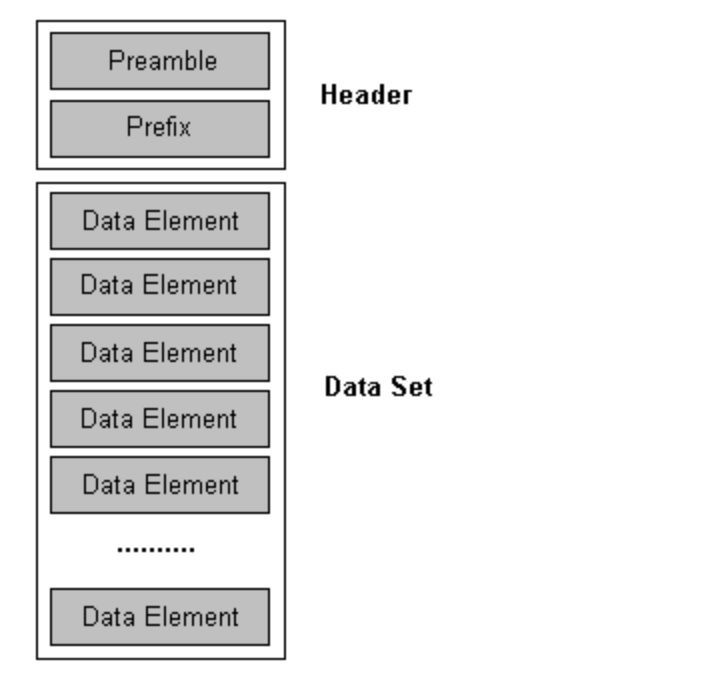
\includegraphics[width = 0.45\hsize]{./figures/DicomFileFormat}
\caption{Basic DICOM File Structure}
\end{figure}

\newline \vspace{5mm}
\textbf{DICOM Data Element} are \textit{Tag Element}, therefore DICOM can be said to be a tag file format, this mean that each element is referenced by a unique \textbf{Tag Number} defining the element and its properties. In the Data Set, Data Elements are ordered by increasing Tag Number. Each Data Element is made of the same range of consecutive fields: 
\begin{itemize} 
\item \textbf{Tag Number}: it consists in an ordered pair of 16 bits unsigned integer of the form (gggg,eeee)  representing the \textit{Group Number} - defining the Information Entity - followed by the \textit{Element Number} - defining the attribute. For example, in the tag (0028,0010), the Group Number is 0028 and correspond to the Image group, the Element Number is 0010 and correspond to the row (especially to the length of the image in pixels).
\item \textbf{Value Representation}: it defines the data type of the element. As the Tag Number already implies the data type, the value representation can be omitted.
\item \textbf{Value Length}: either 16 or 32 bits element, this defines the length of the following value.
\item \textbf{Value Field}: consists in an even number of bytes containing the value of the element; this field can contain the Value Multiplicity, which would specified the number of values that can be encoded in the field. 
\end{itemize}

\begin{figure}[ht]
\centering
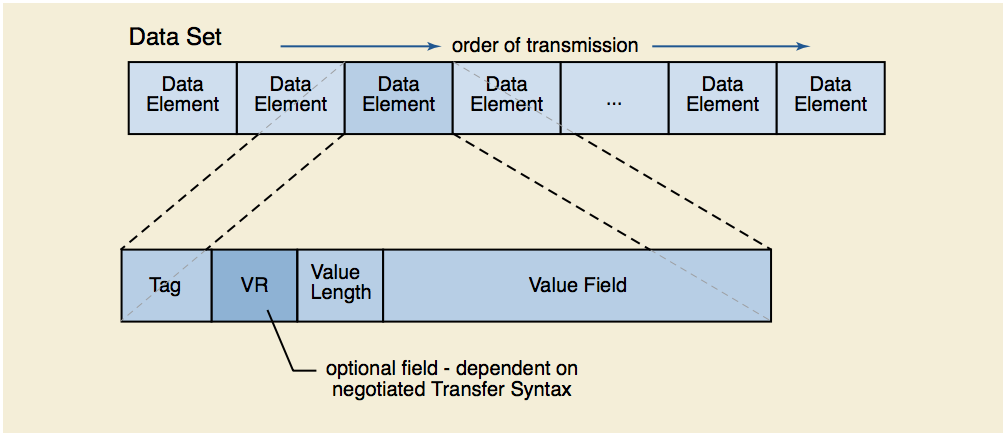
\includegraphics[width = 0.8\hsize]{./figures/DataSetandDataElement}
\caption{Data Set and Data Element structure}
\end{figure} 



\clearpage
\subsection{Choose implementation methods - C++ and Qt}
\input{src/section/groundwork/QtC++}


\clearpage
%%%%%%%%%%%%%%%%%%%%%%%%%%%%%%%%%%%%
\section{Early stage - Creation of a sample interface: display one CT image}
\subsection{An external library to deal with DICOM images: DCMTK}
\textbf{1.What is DCMTK}
\newline
DCMTK is an open-source collection of libraries and applications that has been made to  deals with the DICOM format while developping an independant application. This software is widely used by hospitals, companies or private individuals that aim at creating DICOM related desktop software. DCMTK provide several classes and script in order to treat, construct, and convert DICOM files and an internal worklist server in order store, send or receive images.

\newline
DCMTK source code repository is available on Github and free for downloading. It is available for both Windows and Unix operating systems. For the purpus
 However dcmtk toolkit doesn't came as a prebuilt library 


\clearpage
\textbf{2.DCMTK classes and DICOM Element access}

\clearpage
\subsection{DCMTK classes and DICOM format}
--> DICOM undestanding: more complicated fromat than expected: appdnix for DICOM format explanation
\newline
--> DCMTK installation: see appendix for installation tips + appendix for main classes 
--> Qt tools not so cool

\clearpage
\subsection{A journey to sample interface: building and linking the library}
\input{src/section/earlystage/installation}



\clearpage
%%%%%%%%%%%%%%%%%%%%%%%%%%%%%%%%%%%%
\section{Design and Features Implementation}
\subsection{Time schedule overview}
%Should definitely takl about my issues because project not really reachable
--> provide calendar of project evolution
\newline
-> insert gantt 

\clearpage
\subsection{Main features: development and challenges}
\input{src/section/earlystage/featuresdevelopment}



\clearpage
%%%%%%%%%%%%%%%%%%%%%%%%%%%%%%%%%%%%


\section{FInal Results and Evaluations}
\clearpage
\subsection{Final output}
\input{src/section/results/design}

\clearpage
\subsection{Third party feedback}
\input{src/section/results/patienteval}

\clearpage
\subsection{Personnal evaluation}
--> explain some choice 
\newline
--> show calcul for different plan output

\clearpage
\subsection{Ethic and LSEPI checklist}


\clearpage
%%%%%%%%%%%%%%%%%%%%%%%%%%%%%%%%%%%%
\section{Conclusion and Future work}



\clearpage
%%%%%%%%%%%%%%%%%%%%%%%%%%%%%%%%%%%%
\section{Appendix}
\subsection {Appendix - DICOM Real World Model Structure}

\begin{appendices}
\begin{figure}[ht]
\centering
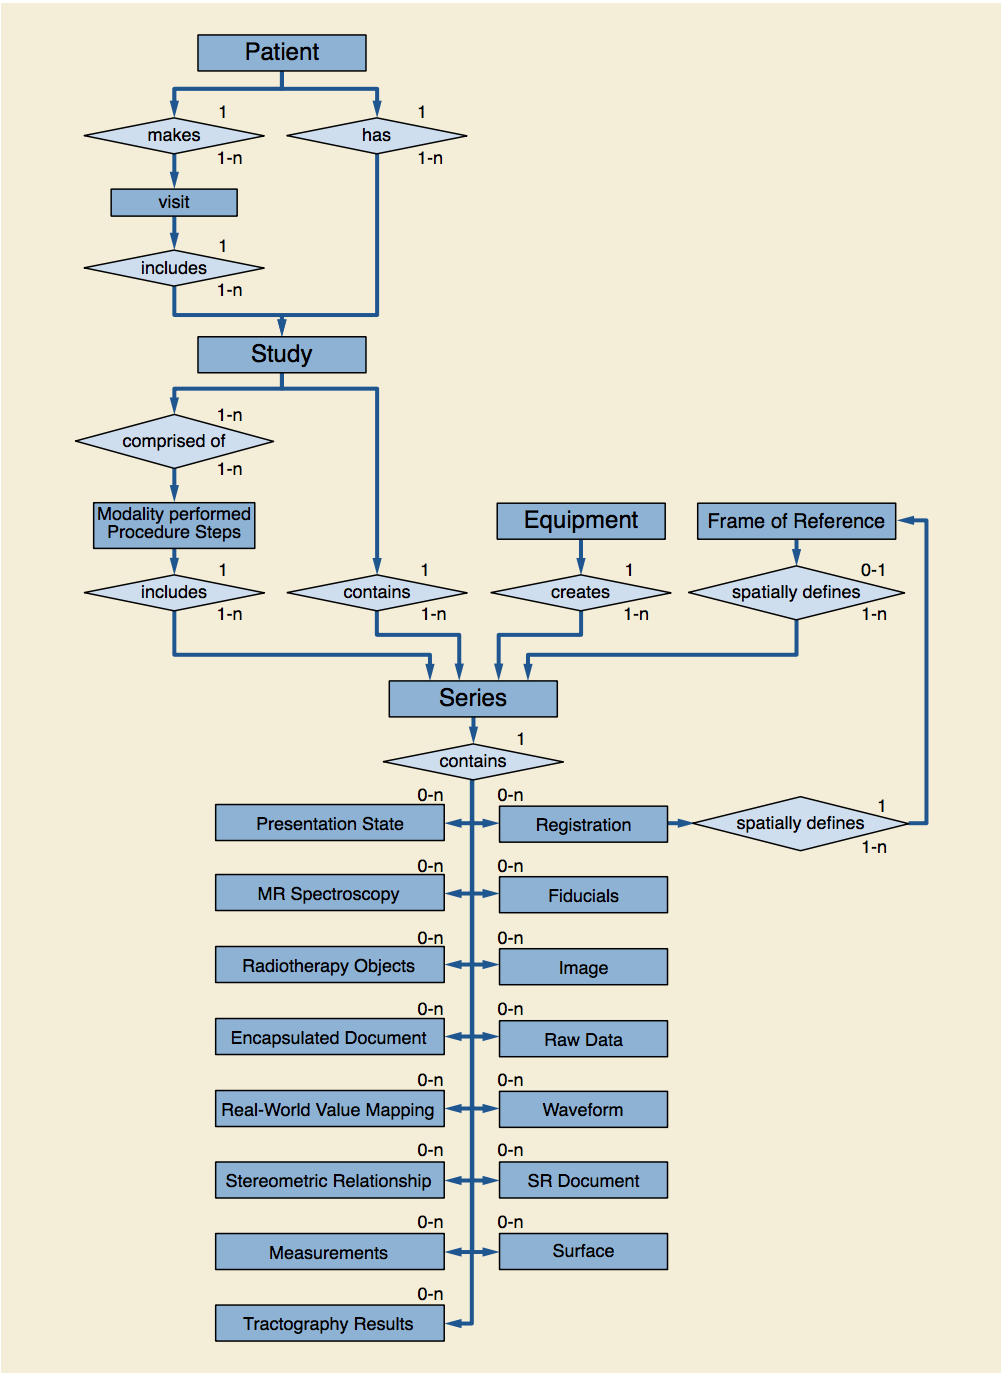
\includegraphics[width = 0.95\hsize]{./figures/DICOMRealWorldModel}
\caption{DICOM Real World Model Structure}
\end{figure}



\clearpage

\begin{figure}[ht]
\centering
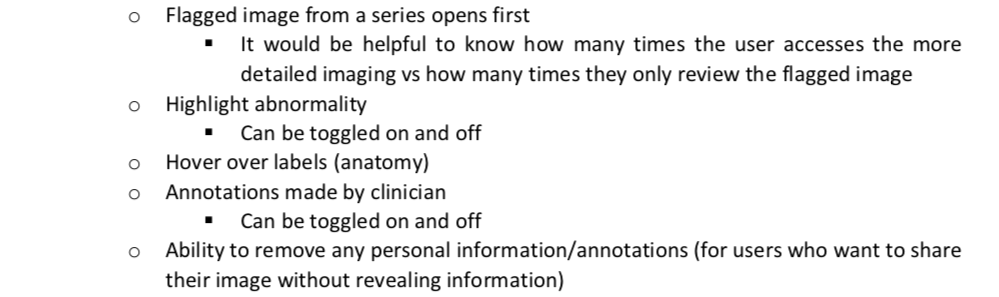
\includegraphics[width = 0.95\hsize]{./figures/GeneralSpec3}
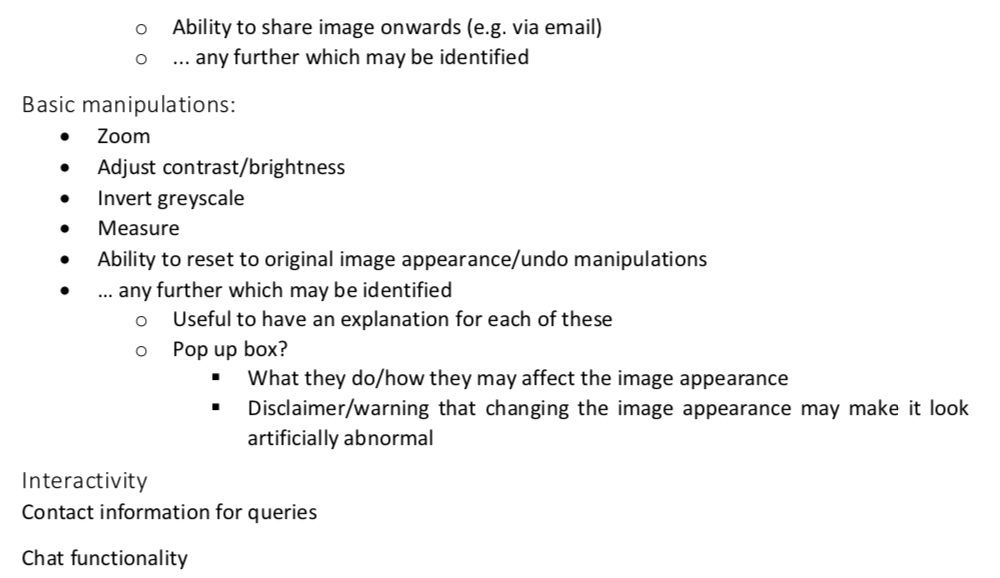
\includegraphics[width = 0.95\hsize]{./figures/GeneralSpec4}
\end{figure}

\clearpage

\subsection {Appendix 2 - Imaging Specification}

\begin{figure}[ht]
\centering
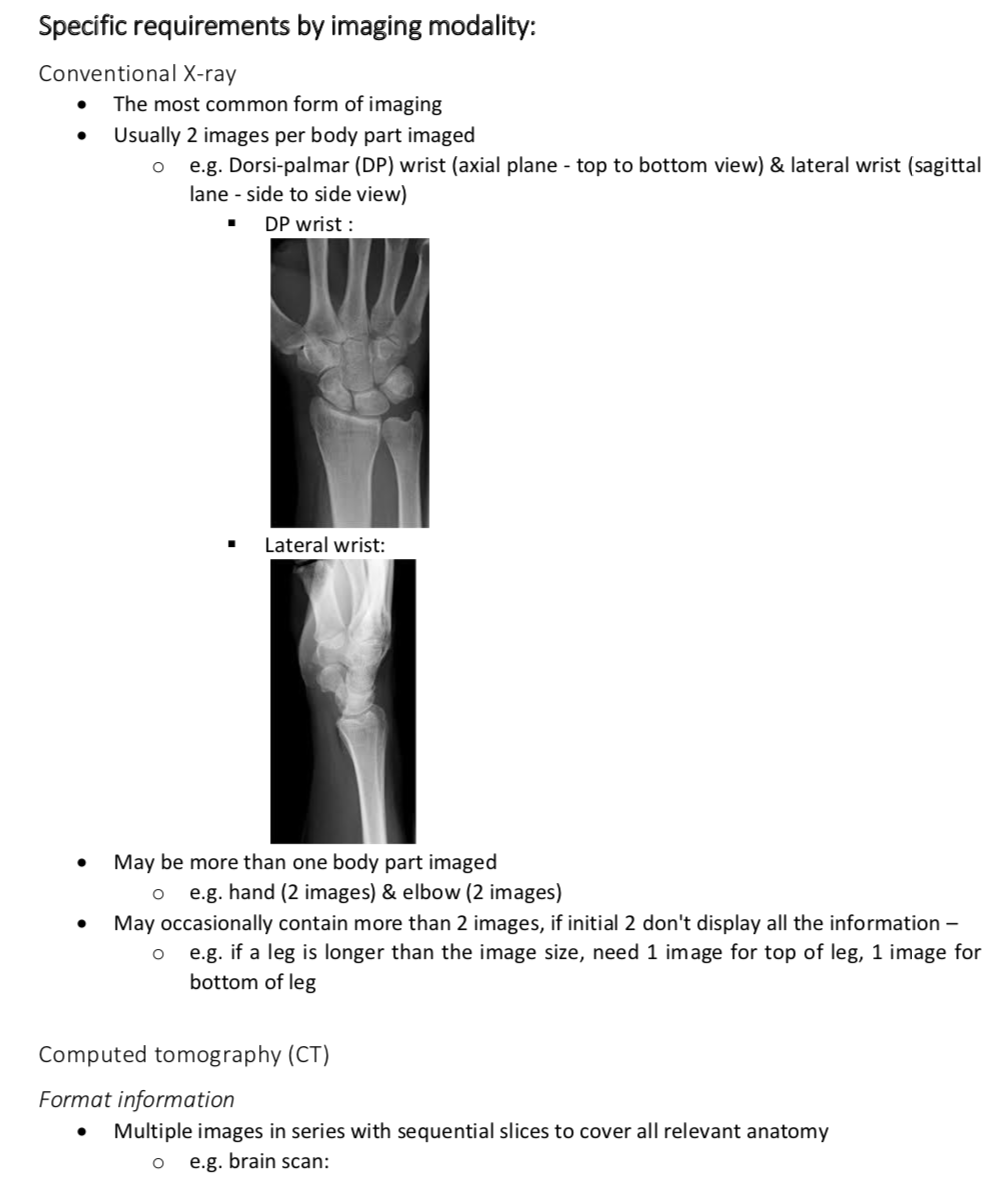
\includegraphics[width = 0.95\hsize]{./figures/ImagingSpec1}
\end{figure}
\clearpage

\begin{figure}[ht]
\centering
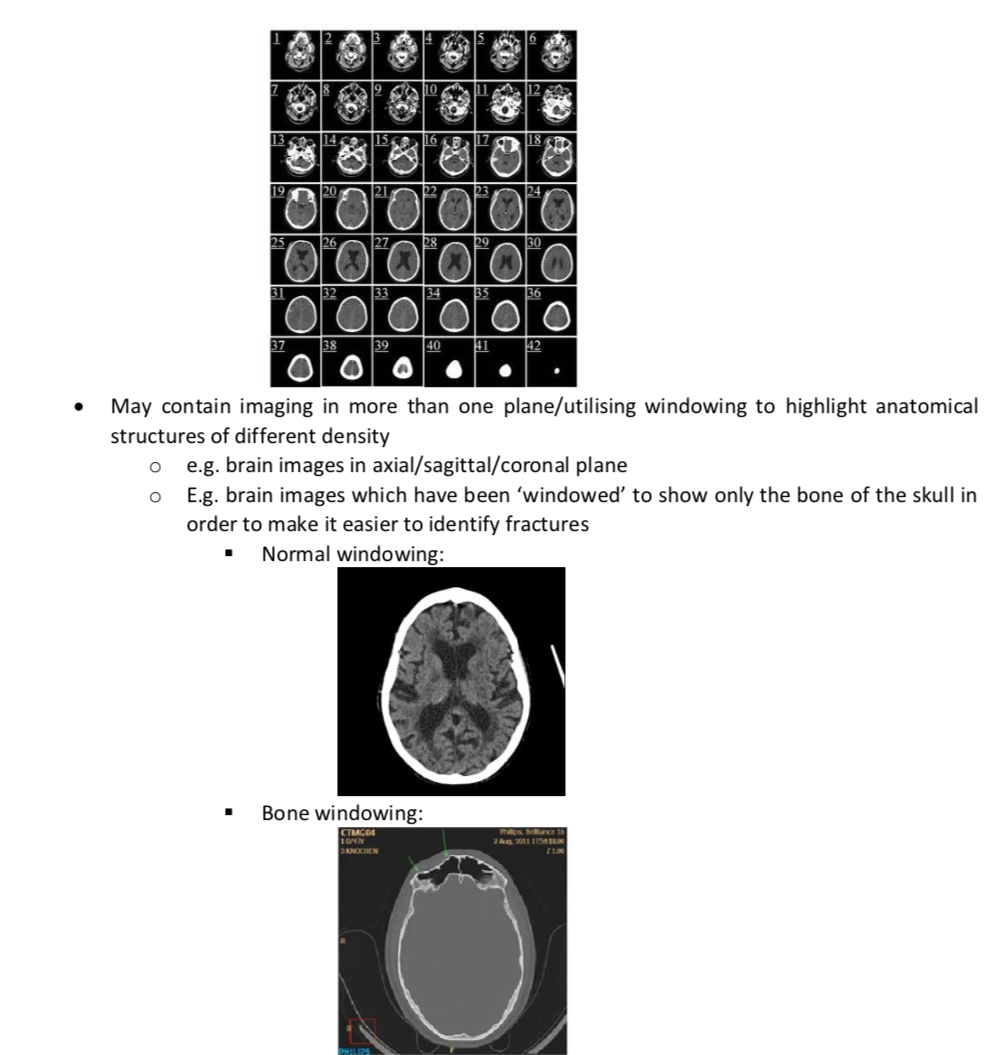
\includegraphics[width = 0.95\hsize]{./figures/ImagingSpec2}
\end{figure}
\clearpage

\begin{figure}[ht]
\centering
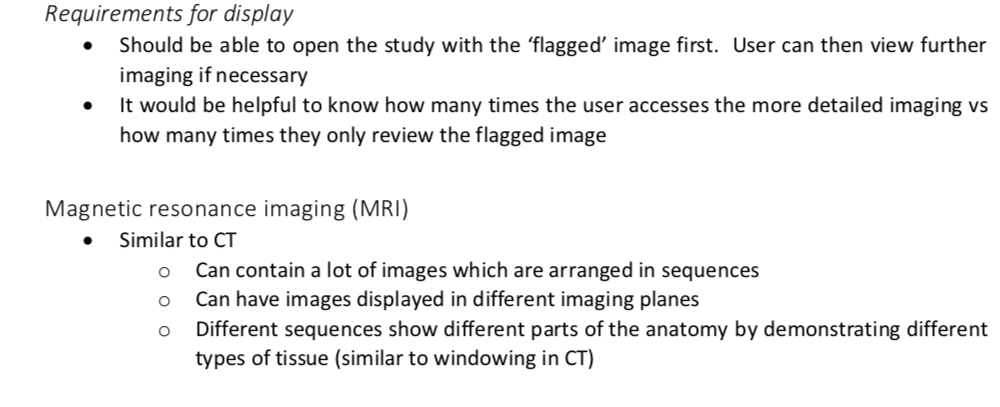
\includegraphics[width = 0.95\hsize]{./figures/ImagingSpec3}
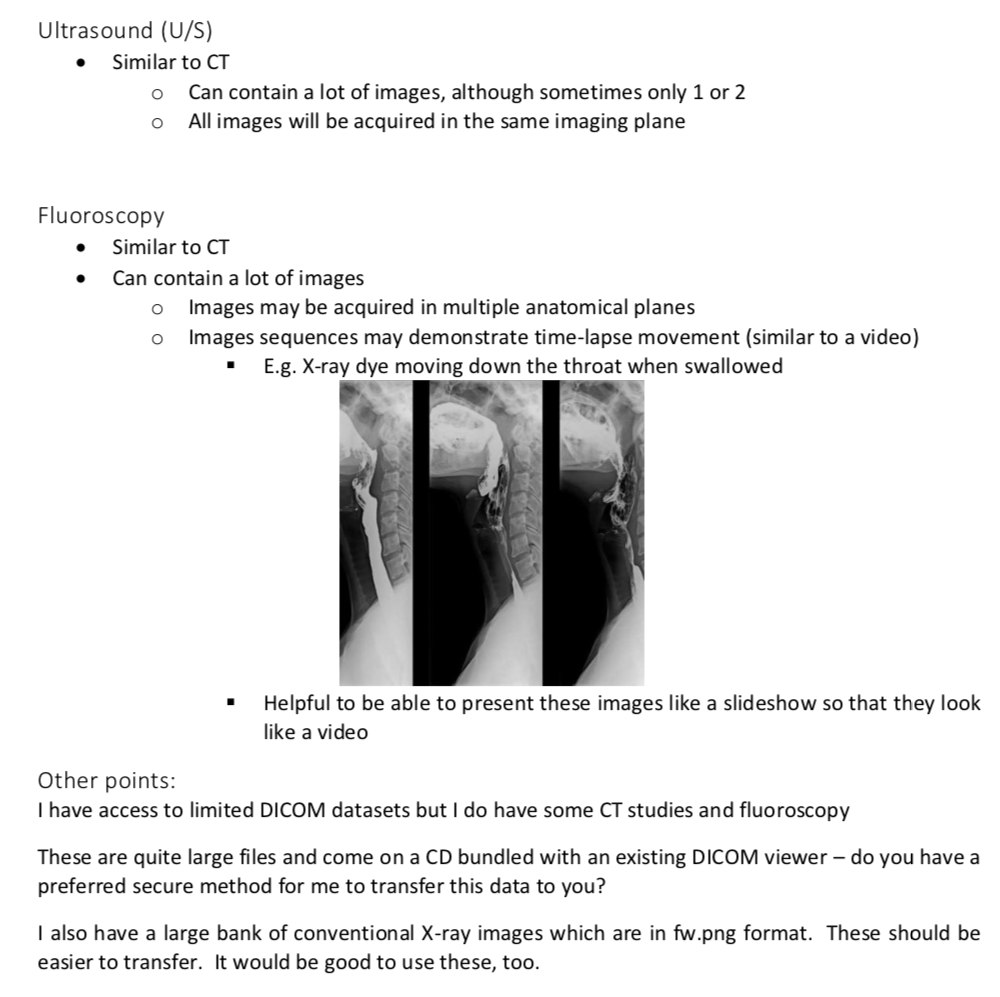
\includegraphics[width = 0.95\hsize]{./figures/ImagingSpec4}
\end{figure}
\clearpage


\subsection {Appendix 3 - Code Overview}



%% bibliography
\printbibliography


\end{document}
